\documentclass{article}
\title{CSC301 HW7}
\author{Alex Zhang}
\date{March 2023}
\textwidth=16.00cm 
\textheight=22.00cm 
\topmargin=0.00cm
\oddsidemargin=0.00cm 
\evensidemargin=0.00cm 
\headheight=0cm 
\headsep=0.5cm
\textheight=610pt
\usepackage{graphicx}
\input zhwinfonts
\graphicspath{ {./images/} }

\usepackage{latexsym,array,delarray,amsthm,amssymb,epsfig}
\usepackage{amsmath}
\usepackage{listings}
\lstset{
  basicstyle=\ttfamily,
  mathescape
}

\newcommand{\bmat}[1]{\begin{bmatrix} #1 \end{bmatrix}}
\newcommand{\mat}[1]{\mathbf{#1}}

\let\ds\displaystyle

\begin{document}
\maketitle
\section*{Question 1}
\subsection*{(a)}
The statement is incorrect by the following counterexample:
\begin{center}
    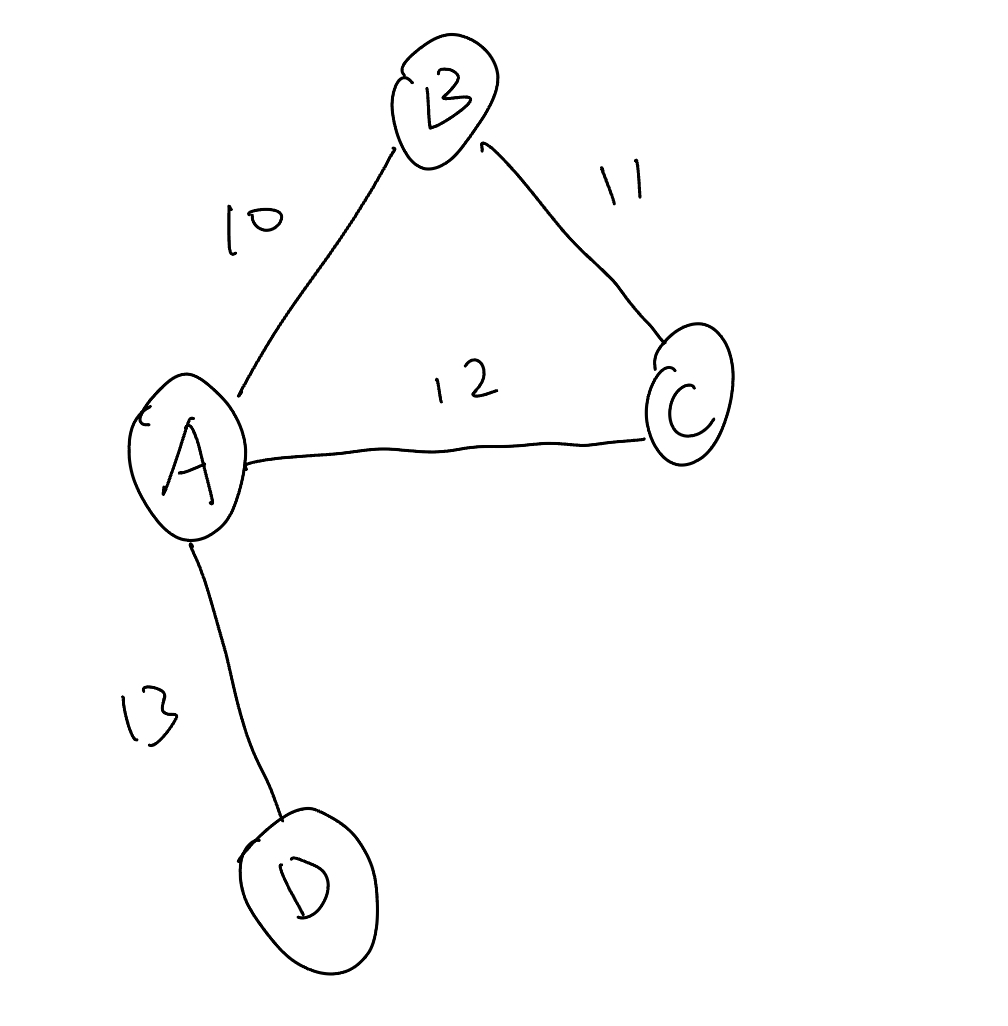
\includegraphics[scale = 0.2]{q1.jpg}
\end{center}
The unique heaviest edge $13$ is in part of an MST (AB, BC, AD).
\subsection*{(b)}
The statement is true. For finding the minimum spanning tree, we have to go through all vertices of the graph.
Assume there are two endpoints that have path contains $e$.
\paragraph*{Case 1:} No cycle between two endpoints

If there is not cycle among these two endpoints, when we have to go through $e$ because there is 
only one path that contains $e$ connects these two endpoints. Therefore $e$ is in the MST.

\paragraph*{Case 2:} A cycle connects two vertices of $e$

If there exist a path other than a path contains $e$ for two vertices, by property of MST, it will remove the
heaviest edge in the cycle and add $e$ instead for creating MST. Because this will create a lighter tree and break
cycle given that $e$ is the lightest edge and unique.

This holds true for every MST because they have to go through two vertices have path containing $e$.

\subsection*{(c)}
The statement is correct.

Assume a subset of edge $X$ which is part of an MST and not include $e$. We can use the cut property
to partition $G$. In this case, we will going to find the lightest edge $e^\prime$ crosses the partition.
We also know that $X \cup e^\prime$ will also be part of that MST.

For each cut, $e^\prime$ is the lightest edge among all possible edges and after the cut, $e^\prime$ is part of an MST.
We can say that if $e^\prime$ is part of an MST, it needs to be the lightest edge for some cut of $G$. It is also true 
for edge $e$ as long as it's in some MST.

\subsection*{(d)}
The statement is incorrect by the following counterexample:
\begin{center}
    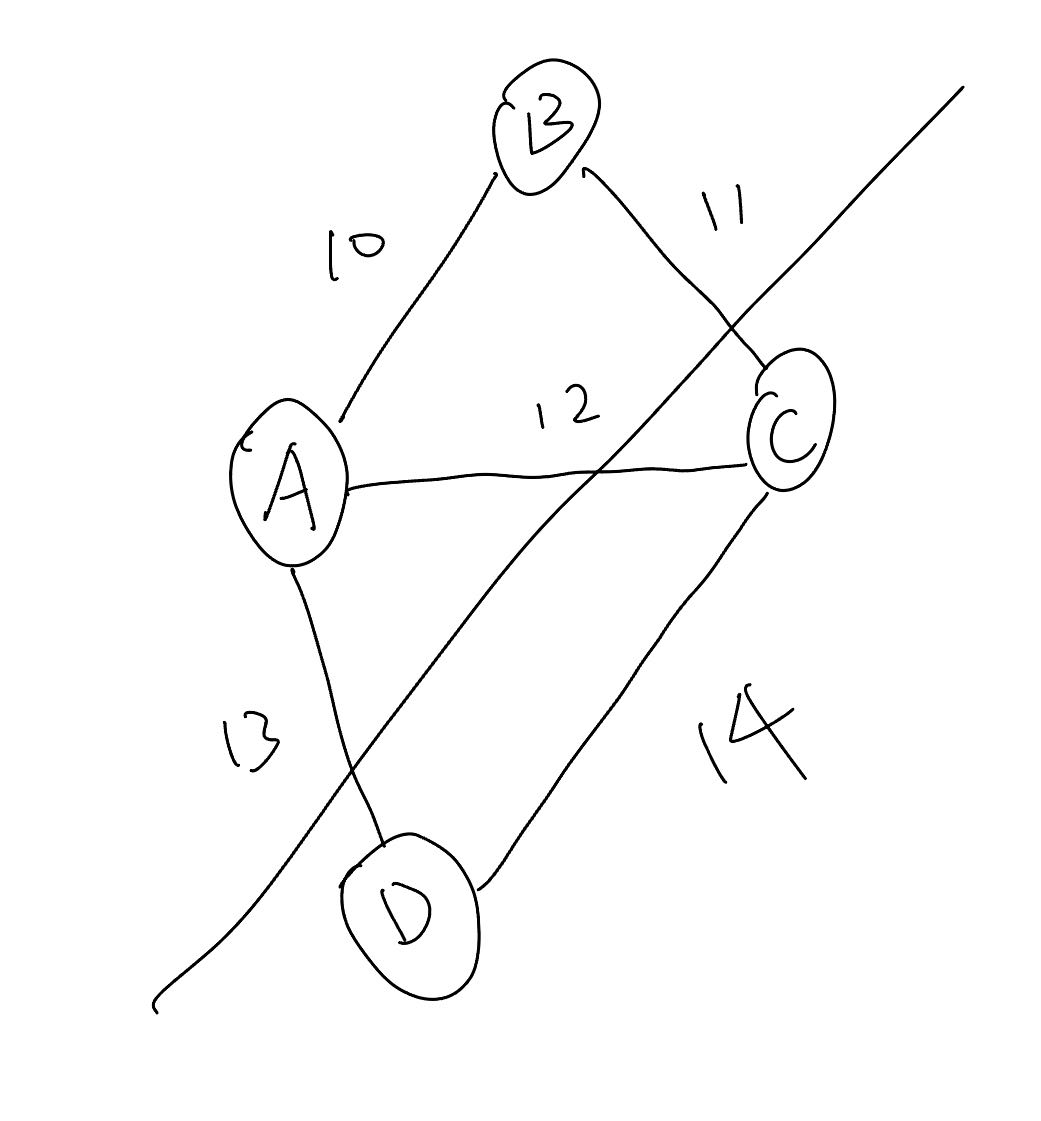
\includegraphics[scale = 0.2]{q1d.jpg}
\end{center}
At first $|V_1|$ is $A$ and $B$, $|V_2|$ is $C$ and $D$. $E_1$ is 10, and $E_2$ is 14. In this case we find edge $e$ to be 11.
With recursion, we will eventually go into base case which for $A$ and $B$, $e$ will be 10, and for $C$ and $D$, $e$ will be 14.

Combining all edges in $E_c$, we find a tree has sum of weights $10+11+14=35$. However, in this graph, the MST has the sum of weights 
with $10+11+13=34$. This divide-and-conquer algorithm will not produce the correct MST.



\section*{Question 2}
The pseudocode of my algorithm:
    \begin{verbatim}
        Function No111(A)
            n = size(A)
            init array dp of size A
            dp[1] = 2
            dp[2] = 4
            dp[3] = 7
            for i = 4 to n do
                dp[i] = dp[i-1] + dp[i-2] + dp[i-3]
            end for
            return dp[n];
        end function
    \end{verbatim}
\subsection*{Proof of Correctness}
Base cases:
\begin{enumerate}
    \item 1-bits string: both "0" and "1" satisfy, therefore dp[1] = 2.
    \item 2-bits string: "00", "01", "10", and "11" satisfy, so dp[2] = 4.
    \item 3-bits string: "000", "001", "010", "011", "100", "101", and "110" satisfy, dp[3] = 7.
\end{enumerate}
Inductive hypothesis:

Assume n-bits string has m1 strings that not include 111, n-1-bits string has m2 strings that not include 111, and n-2-bits string has m3 strings does not include.
We need to show for n+1-bits string, it has $(m1+m2+m3)$ number of string that does not include 111.

For creating any n+1-bits string, it is eccentially adding 0 or 1 in front of a n-bits string.
\paragraph*{Case 1:} Adding 0

If we add a 0 in front of any n-bits string that doesn't include 111, the new n+1-bits string will also not have 111.
Since the maximum consecutive 1's in that n-bits string is 2. Adding a extra 0 will not create three consecutive 1's.

Because we assume that there are m1 number of n-bits string that satisfy this condition, the number of n+1-bits string
will be at least m1.
\paragraph*{Case 2:} Adding 1

In this case the first bit of n+1-bits string will be 1. And there are two cases.
\paragraph*{Case 1:} Second bit is 0

In this case, this means the first two bits of n+1-bits string is "10". In order to make n+1-bits strings
not have three consecutive 1's, we can add all n-1-bits string that does not include 111 after "10". For this case,
all n+1-bits string satisfy this condition will not have three consecutive 1's. There are total m2 number of strings in this case
as we asuumed. So currently the overall number for n+1-bits is $m1+m2$.
\paragraph*{Case 2:} Second bit is 1

In this case, the first two bits of n+1-bits string will be "11". Since we aim to count the number of n+1-bit strings
that does not include 111. The thrid bit has to be 0 in this situation. Thererfore, the first three bits of n+1-bits strings 
have to be "110". If we could add all n-2-bits string behind "110", it will create n+1-bits string that does not include 111.

We assume that there are total m3 number of n-2-bits strings satisfy this condition. There are also m3 number of n+1-bits strings
in this condition.

Overall, sum all numbers of possible n+1-bits strings, we conclude that there are $m1+m2+m3$ number of n+1-bits strings
that doesn't have substring 111.

In representation of the algorithm, for any bit string of length $n$ where $n \geq 4$, the total number of n-bits string that 
doesn't have substring 111 will be represented as the sum for bit string of length $n-1$, $n-2$, and $n-3$ that also not include 111.

\subsection*{Cost Analysis}

Based on my pseudocode, the initialize of array has linear complexity, and there is a for loop up to length $n$. In the for loop, the addition also costs linear time.
So overall the time complexity will be $O(n+n^2)$, generalized into dominating term, the time complexity will be 
$$O(n^2)$$


\section*{Question 3}
\subsection*{(a)}

The file "knapsack.java" used a 2-D array to store the values and weights.
The space complexity will be $O(nW)$, and it runs in $O(nW)$.
\subsection*{(b)}

The file "knapsackMem.java" used an 1-D array to store the maximumx value.
The space complexity will be $O(W)$, and it runs in $O(nW)$.
\subsection*{(c)}
Both of my programs' outputs fit the result.


\end{document}